\subsection{Sketch}
\begin{figure*}
    \centerline{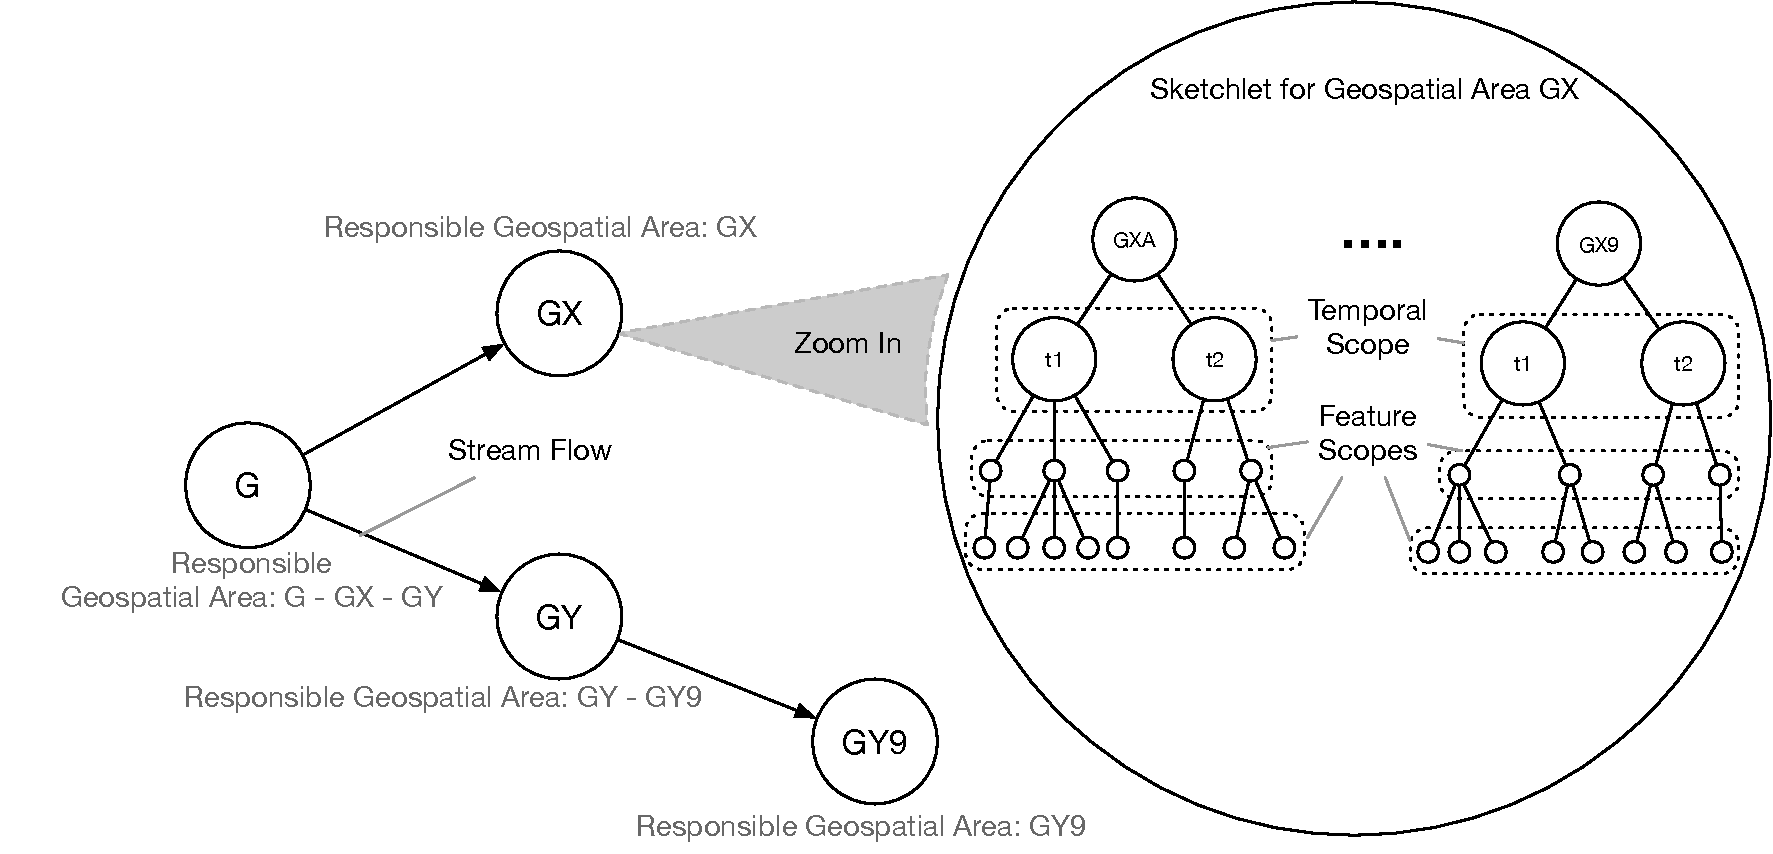
\includegraphics[width=0.8\textwidth]{figures/dist-sketch.pdf}}
    \caption{Demonstration of the distributed sketch for geospatial region with the geohash prefix G. The sketchlets for geohash prefixes GX and GY have scaled out due to high volume of observations. Each sketchlet maintains a SIFT data structure, which is a forest of trees where each tree is responsible for a more specific geospatial region.}
    \label{fig:dist-sketch}
\end{figure*}

The macroscopic view of the distributed sketch is one that comprises multiple sketchlets; each sketchlet executes on a different machine and is responsible for organizing data for a particular geospatial scope. The sketch is organized as a modified, distributed prefix tree. All the descendant nodes -- the sketchlets -- share a common prefix associated with the parent. Unlike traditional prefix trees, where the root node is an empty string, the root node is the coarsest granularity of the geohash i.e. the prefix that is common across all observations. Within a sketchlet all observations share the prefix associated with that sketchlet.

The sketch must be performant and flexible while being amenable to scaling operations. The sketch initiates scale-out operations to relieve memory pressure and preserve performance in the face of voluminous data. Scale-in operations are initiated by the sketch to conserve memory. Any sketchlet may serve as the conduit for incoming queries or analytic operations over the sketched spatiotemporal data: the sketch must be organized such that the sketchlets are not involved in redundant query evaluations or analytic operations. 

The geohash algorithm is well suited to our problem and plays a central role in the organization of the distributed sketch. Since the geohash algorithm represents a bounding box, it facilitates collation of observations from a particular geographical scope. This in turn allows us to redirect queries effectively and ensure data locality during query evaluations. Increases in the length of the geohash string correspond to geographically smaller bounding boxes being identified with increasing precision. This is also well-aligned with dynamic scaling maneuvers performed by the sketch to manage memory requirements and the availability of observational data. Scaling operations within the sketch are targeted. Scale-out operations target geospatial locations with increased density of observations to relieve memory pressure and alleviate performance bottlenecks. Scale-in operations target geolocations where there is a sparsity in available data to conserve memory.

Each sketchlet is responsible for real-time organization, summarization, and compaction of observational data from the geographical scope represented by the sketchlet's geohash.  The sketchlet performs two operations. First, it extracts metadata from incoming observations. Metadata extracted from individual observations include: geolocations, chronological information, and features encapsulated within the observation. Second, the sketchlet is responsible for summarization and compaction of measurements and accompanying spatiotemporal information extracted in the previous step. The sketchlet organizes its summarization of the observational data, as a forest of trees in a data structure called SIFT (Summarization Involving a Forest of Trees). The underlying principle within this data structure is \textbf{grouping} to exploit similarities in values reported within observations. This organization principle extends to all dimensions associated with the observations: spatial, temporal, and encapsulated features. The grouping principle allows us to preserve fidelity of the observational space while conserving memory footprints.

Each tree within the SIFT is rooted at a higher precision geohash than that associated with the sketchlet. For example, at a sketchlet with a geohash prefix, \emph{DJ}, the trees within the SIFT at that sketchlet are rooted at higher precision geohashes such as \emph{DJB}, \emph{DJC}, \emph{DJF}, etc. An advantage of this approach is that the sketchlet partitions data from different regions within the larger geospatial scope into smaller regions. This partitioning allows the data structure to further exploit similarity in the observation values reported for that spatial scope. 

Within each SIFT, the second level is used to group observations based on their temporal properties. This approach allows us to exploit similarity in readings reported for a particular time range. Note that as the trees are traversed, this organization strategy means that all descendants of a temporal node correspond to measurements reported for a particular region and for a particular temporal scope. The SIFT data structure also supports finer-grained temporal resolutions for the recent past -- e.g., minutes, hours, day, weeks, etc. -- along with targeted compaction operations that fold finer-grained temporal scopes into a coarser grained scopes as time advances. Specifically, our organizational structure that allows us to support varying levels of expressiveness for different temporal scopes, with recent observations represented more expressively. For example, on 3/2/2017 we may maintain subtrees at the minute level for 3:01 pm, 3:02 pm, etc., at 3/2/2017 @ 5:00 pm these subtrees will be folded into observations for the hourly temporal scope for 3:00-4:00 pm, and at 4:00 pm the next day (3/3/2017) these would then be folded into the coarser gained temporal bin for the previous day. 

The grouping concept also extends to individual features. Each feature occupies a level within an individual tree in SIFT. At each level, the range of values that a feature can take is broken up into a set of bins (corresponding to the range of values) that they take. These ranges are determined using kernel density estimation (KDE) to ensure that the binning of features is representative of the observed density in the distribution of values for that feature at the particular spatiotemporal scope. Each node (or bin) maintains the min, max, standard deviation, mean, and the total number of observations it is responsible for.  This is useful during the creation of synthetic datasets that are representative of the observational space for a particular spatiotemporal scope. A simplified version of the distributed sketch for geospatial region \emph{D} is depicted in Figure~\ref{fig:dist-sketch}. 

Our methodology of grouping and organizing the summarization information as a forest of trees accomplishes two key objectives. First, it captures the distribution of feature values across a spatiotemporal scope. Second, it supports targeted reductions in the observational data volumes while being representative of the observed feature values. This is in contrast to a random sampling scheme, which may be unable to recreate distributions with high fidelity for arbitrary spatiotemporal scopes or may drop significant values.

The organization of the sketchlet is such that it is amenable to scale-out and scale-in operations of the distributed sketch. Perhaps the most important feature provided by the SIFT data structure is support for scaling operations. For example, if a subregion represented by a tree within the forest maintained at each sketchlet has a higher density (and variability) of the reported observational values, that tree would have a correspondingly disproportionate memory footprint within the data structure. This allows us to target scaling maneuvers to particular subregions managed at a sketchlet to alleviate memory pressure.  During scale-in operations, descendants can be folded into the parent; the descendant's SIFT is simply added as a tree to the SIFT maintained at the parent.
